\section{Trajectory Planning}

At this step, given the points of the desired path, a more detailed trajectory is calculated, 
which will contain all the waypoints that the robot will have to visit. Trajectory planning is executed after a desired path is generated,
and consists in mapping the geometric points to specific time points, as well as assigning specific velocities, accelerations and jerks, 
in order to generate the commands needed for the robot controller to execute a smooth motion.

\subsection{Trajectory planning in cartesian coordinates}

Connect the points from path planning with line segments and add more points if needed

\begin{center}
\begin{figure}[H]
\centering
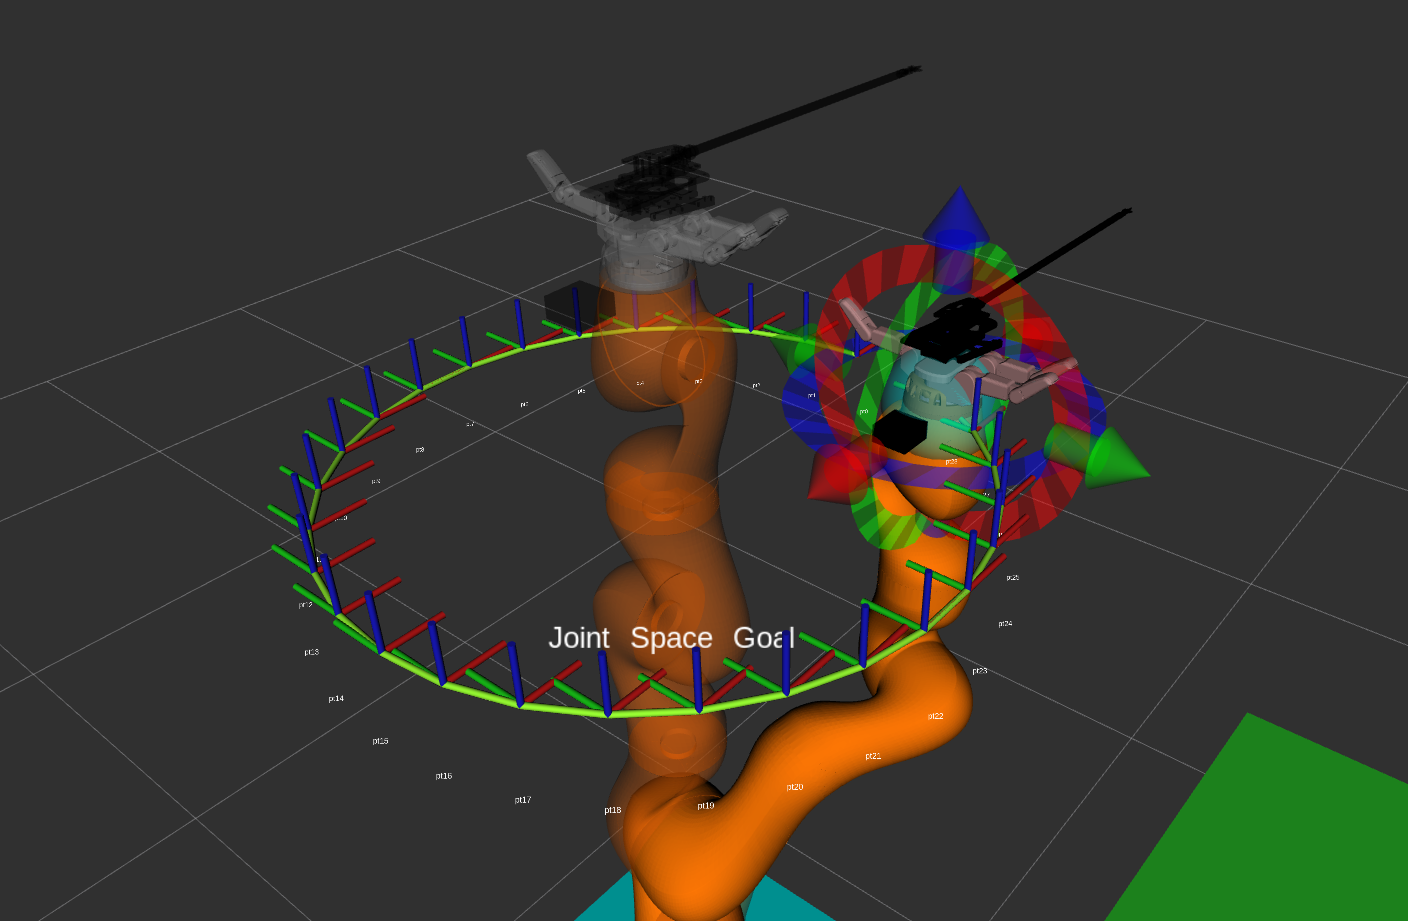
\includegraphics[width=0.7\textwidth]{images/simple_circular_traj1.png}\\
\caption{Circlular trajectory around the z axis of the home position of the robot}
\label{fig:circ-traj-out-of-angle-range}
\end{figure}
\end{center}

It is very important that the designed trajectory respects the joints angles' range. For example
depending on the starting position of the circular trajectory depicted at figure 
\ref{fig:circ-traj-out-of-angle-range}, the robot arm may reach it's joint bounds and in order to 
continue executing the trajectory it will have to make a sudden jump to reset the angles. 
This could have serious side-effects for both the surgical task and thus the patient, as well as 
for the operating staff, who control the robot.

\subsection{Trajectory planning in joint angles space}

\begin{center}
\begin{figure}[H]
\centering
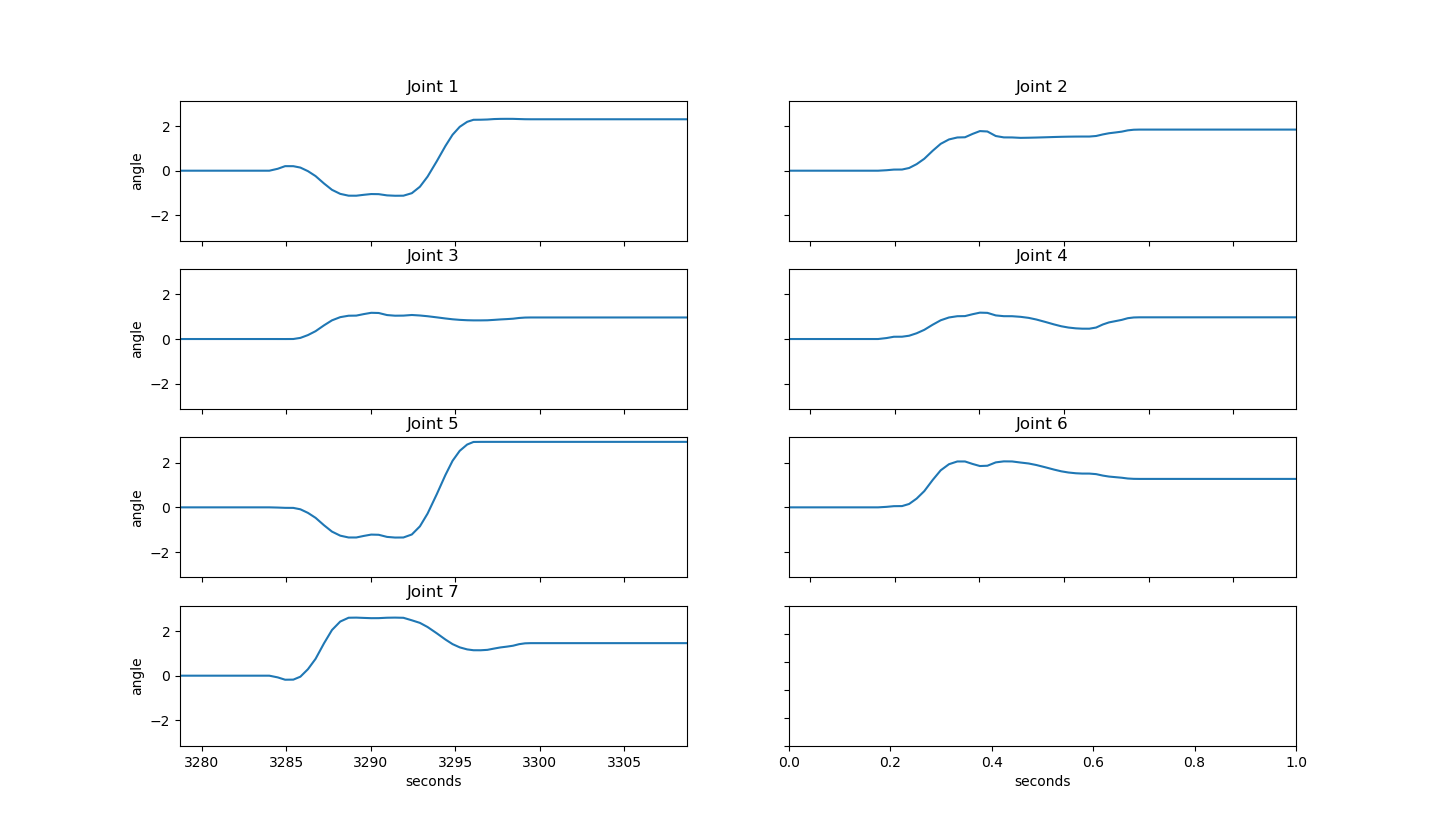
\includegraphics[width=\textwidth]{images/trajectory1-test1.png}\\
\caption{Trajectory diagrams in joints space.}
\end{figure}
\end{center}